\section{Deuxième semaine : Concrétisation de l'atelier}

  Durant la deuxième semaine, nous avons commencé à préparer le contenu nécessaire pour l'atelier. Il a alors choisi d'organiser l'atelier comme un jeu de type \textit{escape game} comportant près d'une dizaine d'énigmes pour les élèves. Au cours de ces énigmes, les élèves devaient deviner un code secret pour accéder à la suite de l'histoire que nous leurs contions et aux énigmes suivantes. Il y a donc eu deux catégories successives d'éngimes. D'abord des énigmes dites \textit{théoriques} qui sont vouées à expliquer le fonctionnement élémentaire d'un modèle de langage, puis des énigmes dites \textit{pratiques}.


\subsection{Partie théorique}

  La partie théorique de l'atelier a été assez simple à concevoir, surtout dans la mesure où elle repose en partie sur le travail de nos prédécesseurs. En effet c'est la deuxième année consécutive que l'\enseirb organise cet atelier de découverte, et nous avons pu nous appuyer sur les travaux réalisés par les étudiants de l'année précédente. Nous avons donc pu récupérer certaines énigmes et les adapter à notre propre approche, tout en les adaptant aux thème de notre atelier. Il a toutefois paru diffile de trouver le juste équilibre entre des énigmes trop simples et des énigmes trop complexes, c'est pourquoi nous avons décidé de choisir de ne pas lésiner sur la difficulté des énigmes, dès lors que celles-ci ne requièrent pas de connaissances mathématiques trop avancées.

  Par exemple, l'une des premières énigmes consistait pour les élèves à découvrir la formule du produit matriciel. Bien que d'apparence cette énigme puisse paraître difficile\footnote{le produit matriciel relevant à ce jour du niveau Terminale option \textit{Mathématiques expertes}}, comme illustré en figure \ref{fig:e3} elle a été conçue de manière à ce que les élèves puissent la résoudre en utilisant uniquement leur logique et leur intuition, sans avoir besoin de connaissances mathématiques de cet ordre. On voit ici que les flèches rouges symbolisent les facteurs à multiplier deux à deux, et que les flèches bleues désignent les termes à additionner. Il faut alors aux élèves comprendre que les lettres doivent être associées à leur numéro dans l'alphabet. Ce qui leur permettra d'obtenir le mot de passe qui est \textit{OPEN}.\par

\begin{figure}[H]
  \centering
  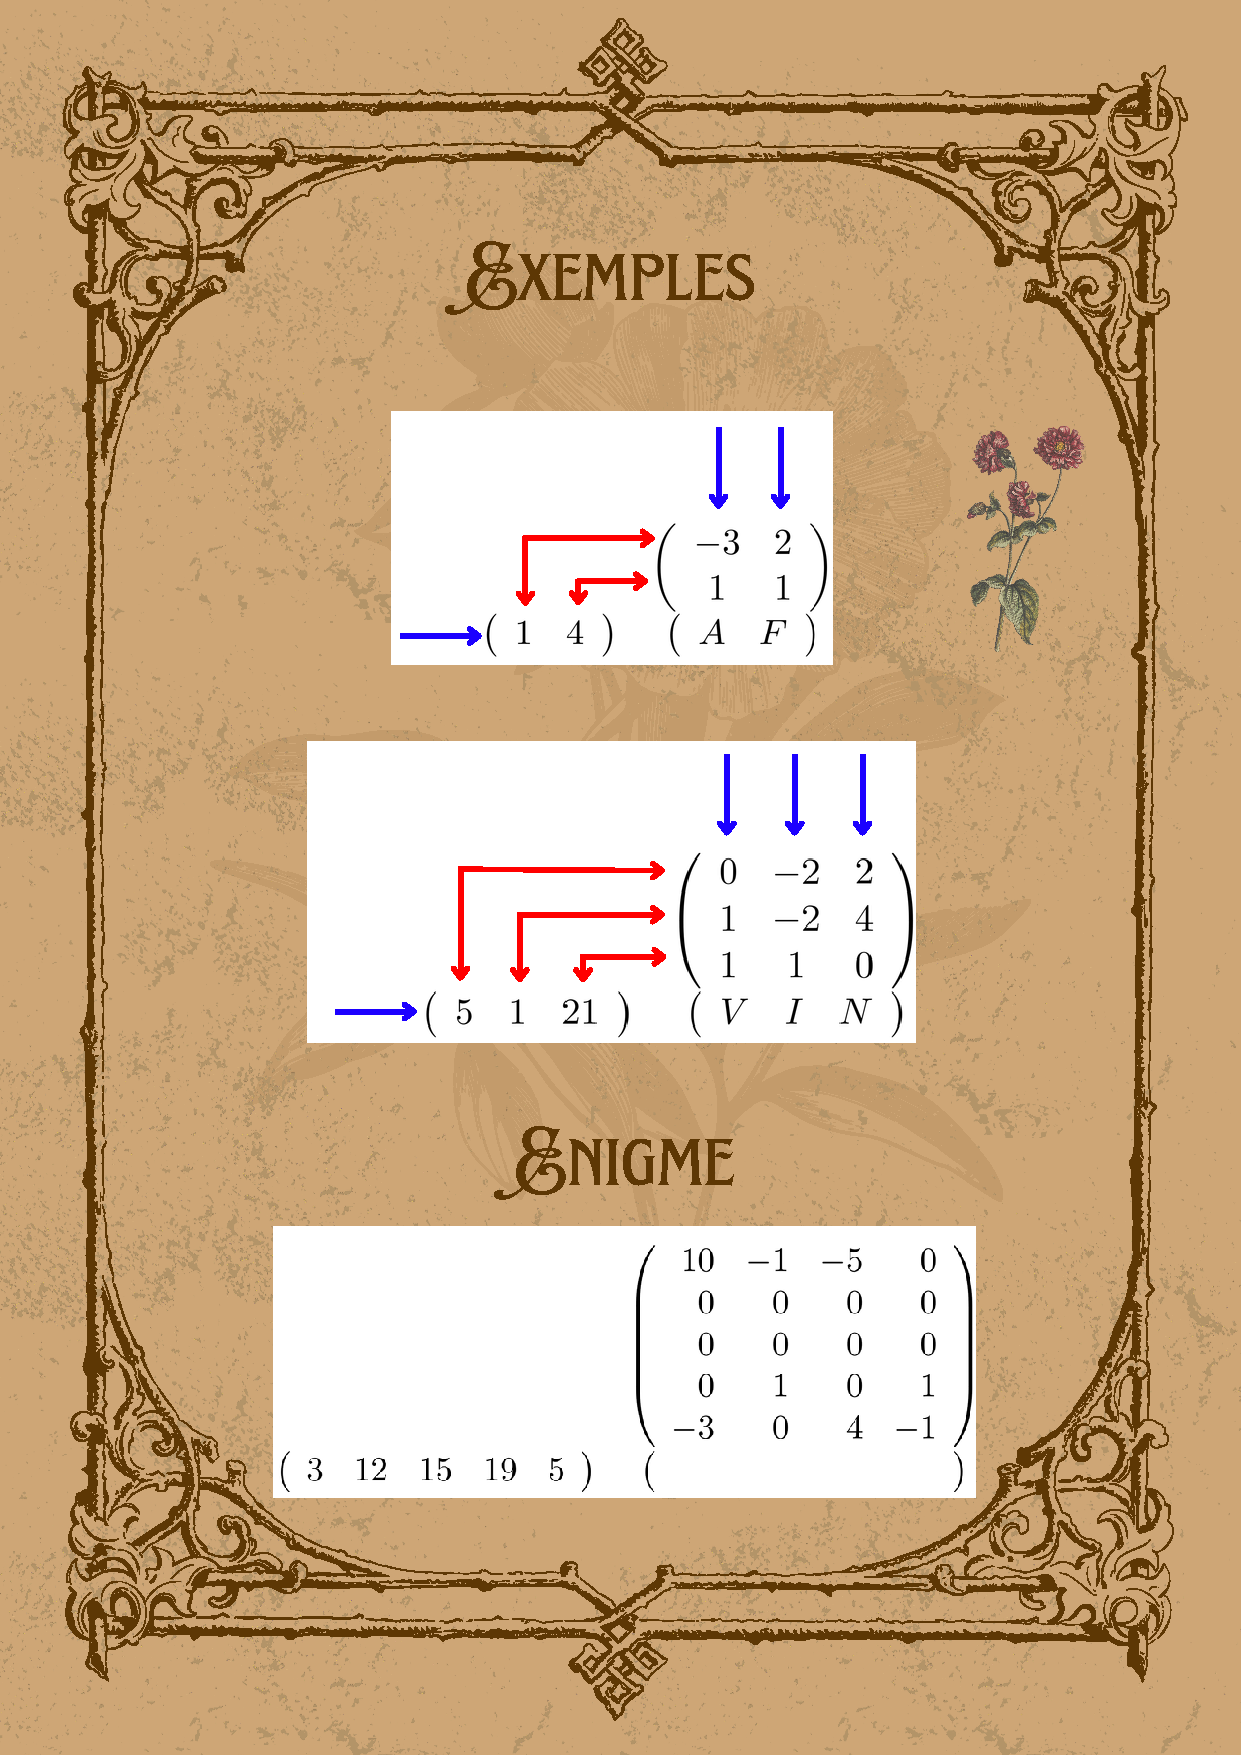
\includegraphics[width=0.5\textwidth]{figures/e3.pdf}
  \caption{Énigme du produit matriciel.}
  \label{fig:e3}
\end{figure}

\subsection{Partie pratique}
  La partie pratique de l'atelier a été plus difficile à concevoir, car elle nécessitait notamment pour les élèves de pouvoir communiquer avec un modèle de langage de sorte que l'interface soit comparable à celles que propose les outils d'intelligence artificielle grand public. Nous avons été octroyés un accès à la machine \textit{Deeeirb} qui est destinée aux tâches associées à l'intelligence artificielle et qui est hébergée par l'école. Nous avons donc pu installer un modèle de langage sur cette machine et le configurer pour qu'il soit accessible aux élèves via une interface web. \par
  Ayant été en charge de l'interface web, j'ai pu acquérir des connaissance sur le développement web, notamment pour la conception d'une énigme dans laquelle les deux élèves sont chacuns face à la même question et doivent y répondre en même temps. Leurs réponses sont alors mélangées avec d'autres écrites par le modèle qui tourne sur la machine Deepeirb, et chacun.e doit retrouver la réponse de son associé.e. Une telle fonctionalité relève de la programmation concurrente car il faut au serveur attendre que les deux élèves et le modèles aient envoyé leur réponse.\par

\subsection{Phase de test, ajustement et biais du modèle}

  Nous avons également eu l'occasion de tester l'atelier avec nos camarades qui préparaient d'autres ateliers pour les élèves de seconde, afin de recueillir leurs impressions et de voir comment ils réagissaient aux différentes activités proposées. Cette phase de test a été très utile pour ajuster le contenu de l'atelier et pour s'assurer que les élèves comprendraient bien les concepts abordés. \par 
Nous avons pu constater que le modèle utilisé pour l'atelier présentait des biais importants, notamment impliquant la formulation de la question qu'on leur pose. En effet le modèle tend à suivre la forme de la question, et à aller dans son sens, ce qui pose problème lorsqu'une réponse objective, indépendante de la question, est attendue. Les biais d'un modèle reposent également grandement sur le fait que leur fonction première est de répondre. Dans un but commercial, un modèle ne doit pas faire d'aveu de faiblesse. Il doit répondre quelque chose, même s'il n'a jamais été entraîné à donner la bonne réponse dans un cas précis. C'est alors qu'il va \textit{halluciner}, c'est-à-dire en pratique répondre quelque chose de crédible mais le plus souvent de faux ou incohérent. \par
Ces biais sont d'autant plus importants que le modèle est vieux. En effet celui-ci date de juillet 2024. Les modèles plus actuels sont beaucoup plus performants et présentent moins ce type de biais, mais nous avons préféré garder un modèle assez vieux pour expliquer plus facilement ces biais, qui même encore aujourd'hui peuvent faire surface lors de conversations complexes avec des modèles du commerce.\par


